\documentclass[conference]{IEEEtran}
\usepackage[T1]{fontenc}
\IEEEoverridecommandlockouts
% The preceding line is only needed to identify funding in the first footnote. If that is unneeded, please comment it out.
\usepackage{cite}
\usepackage{amsmath,amssymb,amsfonts}
\usepackage{algorithmic}
\usepackage{graphicx}
\usepackage{textcomp}
\usepackage{xcolor}
\usepackage{booktabs}
\usepackage{amssymb}
\usepackage{appendix}
\usepackage{hyperref}
\def\BibTeX{{\rm B\kern-.05em{\sc i\kern-.025em b}\kern-.08em
    T\kern-.1667em\lower.7ex\hbox{E}\kern-.125emX}}
    
\begin{document}

\title{ApproxiMPC: Distilling MPCs to LSTMs in F1Tenth}

\author{\IEEEauthorblockN{ Devin DeCosmo}
\IEEEauthorblockA{\textit{Mechanical Engineering} \\
\textit{Carnegie Mellon University}\\
Pittsburgh, PA \\
ddecosmo@andrew.cmu}
\and
\IEEEauthorblockN{ Regine DeCossard}
\IEEEauthorblockA{\textit{Computer Science} \\
\textit{Carnegie Mellon University}\\
Pittsburgh, PA \\
rdecossa@andrew.cmu}
\and
\IEEEauthorblockN{ Henry Feldhaus}
\IEEEauthorblockA{\textit{Mechanical Engineering} \\
\textit{Carnegie Mellon University}\\
Pittsburgh, PA \\
hfeldhau@andrew.cmu}
\and
\IEEEauthorblockN{ Ria Hegde}
\IEEEauthorblockA{\textit{Electrical Engineering} \\
\textit{Carnegie Mellon University}\\
Pittsburgh, PA \\
rhegde@andrew.cmu}
}

\maketitle

\begin{abstract}
Model Predictive Control (MPC) is widely used in autonomous racing because it produces high-performance control while enforcing system constraints. However, solving an optimization problem at every timestep introduces significant computational overhead, making it difficult to deploy on resource-constrained platforms such as F1Tenth vehicles. This work explores distilling an MPC controller into a Long Short-Term Memory (LSTM) network to reduce runtime cost while maintaining performance. Using a teacher-student approach, data generated from an MPC controller is used to train 2 LSTM architectures to mimic MPC based on sequential observations. The learned policy of these LSTM models was evaluated in simulation against 2 MPC baselines to compare lap times, raceline similarity, latency, and memory usage. The study found that LSTM models can be trained to mimic MPC baselines, but additional improvements in data collection, model training, and metrics should be implemented to further optimize performance before hardware deployment.
\end{abstract}

\begin{IEEEkeywords}
component, formatting, style, styling, insert
\end{IEEEkeywords}

\section{Introduction - Condense}
Autonomous racing requires both fast decision-making and accurate control, while also being constrained by limited onboard computation. In platforms such as F1Tenth, this tradeoff becomes especially apparent, since control policies must run in real time on embedded hardware.

Model Predictive Control (MPC) is a strong approach in this setting because it optimizes control inputs while explicitly enforcing system constraints such as vehicle dynamics and friction limits. This typically leads to high-performance behavior, particularly for objectives like minimizing lap time. However, MPC requires solving an optimization problem at every timestep, which introduces significant computational overhead and limits its practicality for real-time deployment.

Long Short-Term Memory (LSTM) networks provide an alternative by approximating sequential control policies with low inference cost. Because they operate on temporal data, they can model system behavior and generate control outputs efficiently. The main limitation is that they do not explicitly enforce constraints, and their performance depends heavily on the quality of training data.

This work explores distilling an MPC controller into an LSTM policy within the F1Tenth environment. The goal is to retain MPC performance while reducing runtime computation, enabling a more efficient control policy for real-time autonomous racing.

\section{Related Work}

\subsection{Model Predictive Control}

There are a large number of control policies possible within F1Tenth, but the most desirable of these are able to optimize a vehicle's performance for minimum lap time or overall performance. 

Model Predictive Control (MPC) is a commonly used control policy within F1tenth and beyond, as it enables optimal or near-optimal control in real time by optimizing an objective function while considering the capabilities of the system \cite{evans2024unifying}. MPC does this by combining input states and constraints to optimize an objective function, in this case, minimum lap time. Input variables are split between state and control parameters. State inputs include the \textit{x} and \textit{y} position of the vehicle along with its heading angle, $\theta$. The main control inputs are velocity \textit{v}, steering angle $\delta$, and the center line speed $\dot{s}$ \cite{evans2024unifying}. Constraints are applied to the friction between the wheels and the surface, and steering regularization is applied. These techniques ensure the vehicle remains controllable and steering is minimized, allowing for a smoother final solution. The objective function can then be optimized as the car runs in both simulation and reality, maximizing vehicle performance. 

 MPC has been applied for several different use cases within F1Tenth, including general performance and lap time reduction, overtaking and opponent following, and variable friction conditions \cite{cataffo2022nonlinear,bhargav2021track,li2023realtime,nagy2023adaptive}. These MPC applications for F1Tenth use the dynamic bicycle model, allowing for high performance and accuracy with decreased degrees of freedom, DOFs \cite{cataffo2022nonlinear,bhargav2021track,li2023realtime,nagy2023adaptive}.

While MPC is a highly capable control policy, it requires a large amount of computation at run time to calculate the objective, including the input states and constraints. This means that applications, such as F1Tenth, that are limited by computational power need to find workarounds to get performance from MPC. Strategies to optimize MPC for local performance, like offline optimization, reduce the reactivity of the control policy, which can cause issues at high speeds or with dynamic obstacles like opponent vehicles. 

\subsection{Long Short Term Memory Models}

Long Short-Term Memory Models, LSTMs, are a subset of Recurrent Neural Network models, RNNs. Like other RNNs, LSTMs take inputs as a sequence, allowing them to consider temporal inputs and make predictions based on both past and present information \cite{ai6090215}. 

An important architectural part of an LSTM is the presence of forget, update, and output gates, allowing for inputs to be considered only if they are relevant or useful, making them adaptable to noise or errors in input data \cite{ai6090215}.

The modular nature of LSTM blocks also means that a model can be adapted to be lightweight enough to run on edge hardware like Nvidia Jetson Nanos. 

LSTMs have been tested using Formula Student races as training data and found they are robust, but require large amounts of training data \cite{srinivasan2020end}. LSTMs have also been tested on the F1tenth system using public datasets for velocity estimation, and MPC data for overtaking in simulation \cite{wegrzynowski2024learning,zhang2023f1tenth}. 

These results show that LSTMs are trainable and useful for creating control policies within F1tenth. 

\subsection{Transfer Learning MPC to LSTM}

While past studies have used MPC, LSTMs, and even trained LSTMs for specific tasks using data from MPC, none of these have focused on overall racing performance or been tested on a physical F1tenth vehicle. 

Additional work has discussed how MPC data can be curated and used to train LSTMs to mimic MPC performance \cite{munoz2023deep}. Also, more work with the F1Tenth system focused on purely overtaking using LSTMs has also shown that MPC data can be collected and used to train LSTMs \cite{zhang2023f1tenth}.

These past works demonstrate that an existing MPC control policy can be used to collect racing data and train an LSTM to approach optimal performance. The moderate parameter size of LSTMs also ensures that training can be done efficiently, while still generalizing across race situations. 

\section{Methods}

\subsection{Data Collection Workflow}
% Focus on the workflow for the data we DID use, not everything we did

% - Gym-Khana with stmpc, access to centerline

% - talk episodes, forward/reverse, maps, speeds, binned lidar, curvature-based lookahead, etc

% - talk about periodic noise resulting from misaligned controller/sim timesteps

% - logging package for both mpc and lstm captures state, and computes/latency metrics

Training data was collected in Gym-Khana \cite{gymkhana_repo2026}  using the included STMPC controller as the expert teacher policy. Gym-Khana was used because it provided fast closed-loop simulation, configurable map sweeps, and direct access to the track centerline, which allowed each transition to be labeled with both local vehicle state and map-relative path context. The collection was driven by YAML configuration files specifying the map set, driving direction, episode count, perturbation settings, LiDAR processing, and lap termination logic. Each map was run in both normal and reverse directions to increase trajectory diversity. At each 10 ms timestep, the logger stored the vehicle state, expert action, executed action, episode and step identifiers, collision/boundary flags, and a min-pooling 60-bin LiDAR vector. In subsequent collection runs, data was augmented with centerline curvature lookahead at 1, 2, 3, 5, and 8 m ahead of the vehicle, giving the learned controller a limited preview of upcoming turns without passing the full centerline.

Two dataset versions were used, see a summary of the differences in Table~
\ref{tab:dataset_collection}. \textbf{Dataset V1} served as a prototype for validating the training pipeline and smoke-testing the LSTM formulation. It covered 7 bidirectional maps with 10 episodes per map-direction pair, producing 140 episodes and 1.41 million transition datapoints. V1 used relatively large one-timestep steering perturbations with 25\% occurrence probability, which helped verify recovery labeling functionality but produced limited sustained off-center correction behavior. \textbf{Dataset V2} expanded the collection to 25 bidirectional maps with 15 target episodes per map-direction pair, for a planned 750 episodes. The final accepted set contained 725 clean episodes and 10.13 million transition datapoints; the shortfall came from Montreal normal, Montreal reverse, and Yas Marina normal, exhausting the retry budget.

\begin{table}[htbp]
\renewcommand{\arraystretch}{1.2}
\caption{Dataset Collection Summary}
\label{tab:dataset_collection}
\centering
    \begin{tabular}{lcc}
        \hline\hline
        \textbf{Attribute} & \textbf{Dataset V1} & \textbf{Dataset V2} \\
        \hline
        Maps & 7 & 25 \\
        Directions & Normal, reverse & Normal, reverse \\
        Map-direction combos & 14 & 50 \\
        Complete combos & 14 & 47 \\
        Target episodes & 140 & 750 \\
        Generated episodes & 140 & 725 \\
        Transition datapoints & 1.41M & 10.13M \\
        Perturbed datapoints & 58,863 & 305,189 \\
        Perturbed fraction & 4.17\% & 3.01\%$^{\mathrm{a}}$ \\
        Lidar features & 60 bins & 60 bins \\
        Curvature lookahead & No & 1, 2, 3, 5, 8 m \\
        Perturb. duration & 1 timestep & 5--25 timesteps \\
        Perturb. magnitude & Large fixed scale & Gaussian steering noise \\
        \hline
        \multicolumn{3}{p{0.92\linewidth}}{\footnotesize
        $^{\mathrm{a}}$ With 25\% perturbation trigger probability, 500-step cooldown, and 5--25 timestep hold duration, there are 305,189 perturbed transitions, or 3.01\% of the final dataset.} \\
        \hline\hline
    \end{tabular}
\end{table}


To improve data quality, V2 retried failed episodes until each map-direction pair either reached its target or exceeded a threshold. It accepted only episodes that completed the target lap count with zero collisions and boundary-violation steps. Unlike V1, V2 used normally distributed steering perturbations held over multiple timesteps while recording both the expert STMPC action and the applied perturbation. This created DAgger-style recovery labels, where the vehicle could be displaced from the nominal trajectory while the target action still reflected the expert recovery policy. The same logging workflow paired state traces with compute and latency measurements, allowing controller timing artifacts from simulator/controller update-rate mismatch to be treated as part of dataset validation rather than only final performance reporting.


\subsection{Model Training Workflow}

As data needs were defined and data were collected, an accompanying model training workflow was defined to reduce delays. Several training assumptions were defined to reduce the design space and focus on comparisons of model size and map performance in a narrow band. LSTMs were chosen as their internal logic gates allowed for automatic rejection of poor or deformed inputs, such as noise in LiDAR scans. The general architecture of the LSTM model is shown in Figure \ref{model_arch}.

\begin{figure}[htbp]
    \centering
    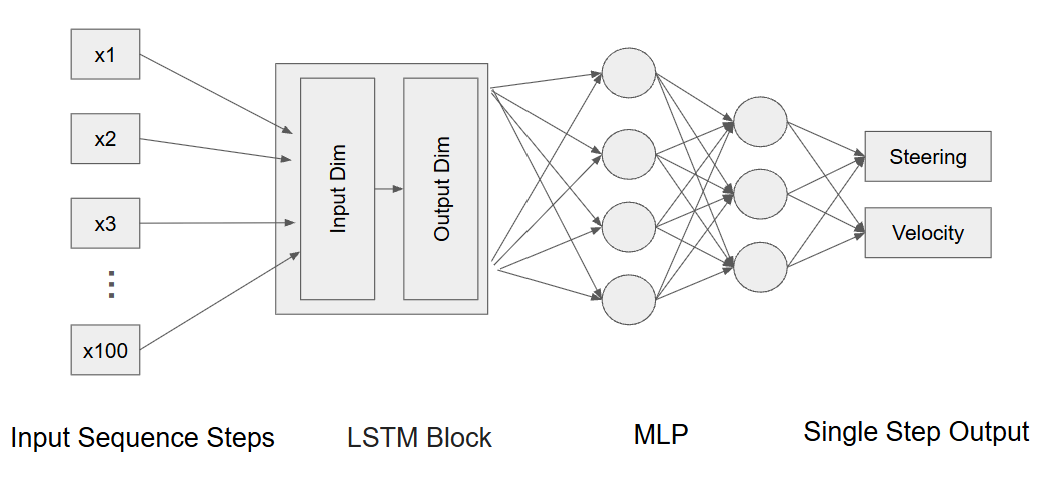
\includegraphics[width=\linewidth]{assets/lstm_diagram.png}
    \caption{General ApproxiMPC Model Architecture}
    \label{model_arch}
\end{figure}

The main training assumptions for this study were that only LSTM models would be considered and that the input sequence length would be 100 steps and the output would be 1 timestep. This made training very consistent and reduced complexity within the scope of the project. 

The rest of the parameters were alterable, including the LSTM hidden dimension, the number of LSTM blocks, and MLP Parameters. 

The standardized input features for the two models considered in this study are listed in Table \ref{tab:feature_comparison}.

\begin{table}[htbp]
    \renewcommand{\arraystretch}{1.3} % Adds standard IEEE vertical padding
    \caption{Comparison of Input Features Between Model V1 and Model V2}
    \label{tab:feature_comparison}
    \centering
    \begin{tabular}{l c c}
        \hline\hline
        \textbf{Attribute / Feature} & \textbf{Model V1} & \textbf{Model V2} \\
        \hline
        \textbf{Dataset} & Dataset 1 & Dataset 2 \\
        \textbf{Total Input Features} & 63 & 68 \\
        \textbf{Past Steering Angle} & Yes & Yes \\
        \textbf{Past Velocity Values} & Yes & Yes \\
        \textbf{Lidar Batches$^{\mathrm{a}}$} & Yes & Yes \\
        \textbf{Curvature Lookahead$^{\mathrm{b}}$} & No & Yes \\
        \hline
        \multicolumn{3}{l}{$^{\mathrm{a}}$Condensed to 60 min input buckets to reduce parameters.} \\
        \multicolumn{3}{l}{$^{\mathrm{b}}$Arc-length distance: 1, 2, 3, 5, 8 meters ahead.} \\
        \hline\hline
    \end{tabular}
\end{table}

The two models used in this study were iteratively trained to refine performance versus the MPC baseline. 

\textbf{Model V1:} Initial mapless model, used to validate data collection and training assumptions, along with identifying early issues

\textbf{Model V2:} Improved Curvature model, used a larger dataset, and map curvature inputs to improve performance for validation and comparison to MPC.

For training LSTMs and other sequence models, there are two possible training methods: teacher-forcing or autoregression. The teacher force passes the correct values at each subsequent time step during training, while the autoregression passes the predictions as input to the next time step \cite{davies2024teacherforcing}.

Due to the high-dimensional inputs and low-dimensional outputs of the LSTM model, the teacher force is the only realistic option for training. This simplifies training, but can make generalization more difficult when the model encounters out-of-distribution data. 

After training using Gym-Khana data, the models need to be packaged and deployed for testing in ROS. The method chosen for this study was to convert all models to ONNX to improve performance without the optimization needed for TensorRT. This served as a baseline case for testing the model. These ONNX models were then called into ROS packages for the control policy tested in the simulation environment F1Tenth Gym. 

\subsection{Evaluation Methodology}
When validating the performance of the distilled LSTM controllers against the expert Model Predictive Control (MPC) policy, our evaluation methodology focused strictly on the workflow for the final accepted data. The validation was divided into two primary branches: Raceline Comparison and Computational Comparison. 

\subsubsection{Raceline Comparison Overview}

To make a fair comparison of the race line, we evaluated the racing performance of the Gymkhana MPC (the baseline teacher) directly against the ROS-deployed LSTM. We selected a suite of five validation maps: IMS, Drift2, BrandsHatch, Spielberg, and Mexico City. This specific set was curated because it scales up in track difficulty, introducing increasingly complex features such as tight hairpins to push the limits of the controllers. The set included both tracks present in the training data and novel tracks to test the model's ability to generalize. 

Additionally, to quantify how similarly the neural network understood the track compared to the teacher algorithm, we calculated the path similarity using spatial interpolation. Rather than comparing states based on the elapsed time, which would skew the results if one controller drove faster than the other, w e compared the exact coordinates $X$ and $Y$ based on the cumulative physical distance traveled. This approach provides a mean spatial similarity metric, explicitly measuring how far apart the corresponding points on each path are from each other in meters on average.

For computational validation, comparing the simulated Gymkhana Python MPC against an ROS-based neural network introduces environment-level timing artifacts. Specifically, ROS LSTM and Gymkhana MPC are not directly comparable computationally because Gymkhana utilizes a fundamentally different underlying optimization solver. Therefore, implementing a separate ROS-based MPC was necessary to serve as an accurate 1-to-1 baseline to evaluate true computational overhead and latency.

\subsubsection{Computational Comparison Overview}

For computational validation, comparing the simulated Gymkhana Python MPC against an ROS-based neural network introduces environment-level timing artifacts. Specifically, ROS LSTM and Gymkhana MPC are not directly comparable computationally because Gymkhana utilizes a fundamentally different underlying optimization solver. Therefore, implementing a separate ROS-based MPC was necessary to serve as an accurate 1-to-1 baseline to evaluate the true computational overhead. We isolated this overhead by running both the ROS-based MPC and the ROS LSTM on a subset of two validation maps. 

To provide a holistic understanding of the computational demands and evaluate their suitability for embedded edge hardware, we defined and measured three distinct performance metrics along with the overall memory footprint:

\begin{itemize}
    \item \textbf{End-to-End Callback Latency:} The total real-time duration required for the ROS node to receive incoming state data, process it, and publish the resulting control command.
    \item \textbf{Core Compute Time:} The isolated execution time of the mathematical algorithm itself, specifically, the forward-pass inference of the ONNX network for the LSTM, and the optimization solver iteration for the MPC. 
    \item \textbf{P95 Latency:} The 95th percentile of callback times. Tracking this bounds the worst-case execution delays, ensuring the controller is consistent enough to safely operate at 100 Hz.
    \item \textbf{Peak Resident Memory (RSS):} The maximum RAM allocated by the node during continuous racing operations.
\end{itemize}

Defining these specific sub-components allows us to move past generalized simulator overhead and measure the true hardware processing requirements necessary for each control step.


\section{Results}

\subsection{Model V1 Results}

The V1 model was used to validate the training and testing assumptions with a mapless method. Another important aspect of Model V1 was determining acceptable model sizes for deployment.

\begin{table}[htbp]
    \centering
    \caption{Performance and Complexity Comparison of LSTM Models}
    \label{tab:lstm_comparison}
    \begin{tabular}{lrcrr}
        \toprule
        \textbf{Model} & \textbf{Parameters} & \textbf{Val RMSE} & \textbf{Steering $R^2$} & \textbf{Velocity $R^2$} \\
        \midrule
        64D LSTM  & 39,826    & 0.018 & 0.879 & 0.986 \\
        128D LSTM & 125,730   & 0.047 & 0.880 & 0.983 \\
        512D LSTM & 1,354,306 & 0.039 & 0.933 & 0.996 \\
        \bottomrule
    \end{tabular}
\end{table}

These results suggest that the larger dimensional models, 128 and 512, have best correlations with output scores. These models were trained in Dataset V1 using teacher forcing. The results from training for the 128 hidden dimension model is shown in Figure \ref{fig:modelV1-training}.

\begin{figure}[htbp]
    \centering
    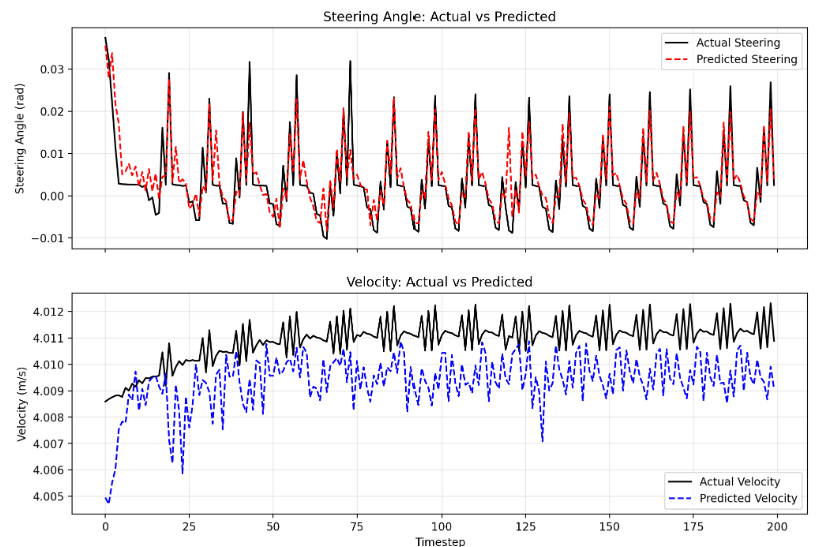
\includegraphics[width=0.7\linewidth]{assets/lstmV1_training.png}
    \caption{Model V1: 128 hidden dimension training results}
    \label{fig:modelV1-training}
\end{figure}

These results demonstrate that the model can fit to a noisy and diverse range of data coming from the Gymkhana MPC. They also demonstrate serious overfitting on the very small pertubations from Dataset V1. The second iteration of the model remedy these errors to improve training and deployment. 


After training was completed, the models were converted to ONNX and run on a set of 5 test tracks of increasing difficulty. 

\begin{table}[htbp]
    \centering
    \capti,on{Model V1 Success Rates by Map}
    \label{tab:model_v1}
    \begin{tabular}{lc}
        \toprule
        \textbf{Map} & \textbf{Model V1 Success} \\
        \midrule
        IMS         & 0/3 \\
        Drift 2     & 0/3 \\
        BrandHatc;  & 1/3 \\
        Spielberg  , & 1itsReverse) \\
        Mexico City & 0/3 \\
        \bottomrule
    \end{tabular}
\end{table}

These results make the V1 model look like a complete failure, as the models were unable to complete many maps without crashing into walls and failing. However, even though the models did fail at some point in most cases, the V1 models were able to approximate a centerline and make adjustments around corners. The failures of the model come down to the training assumptions m. Thisring the model design. It is also important to mention only the 128D and 64D models saw successful runs on individual tracks, the 512D was deemed too large as it's large size and high latency would cause oscillations and crashes on all tracks.

The reduced perturbations of the training data made the V1 models adaptable when close to the centerline, but whenever they would stray far from the centerline they had no method to return to the desired centerline location resulting in crashes on long straights and tight corners. The model itself also, has no information about future track features beyond the LiDAR scans as inputs, this makes identifying features like hairpin corners or chicanes difficult since they are based solely on LiDAR inputs. This made V1 a good proof of concept for the methods for collecting and training these LSTMs and improvements were made to create a more robust and useful V2 model .

\subsection{Model V2 Results}

These lessons from Model V1 were applied to Dataset V2 and Model V2 to improve performance versus the MPC baseline. The main changes to V2 were the use of the V2 dataset that was 10 times larger than the orignal with larger perturbations and the inclusion of lookahead sequence values as input to the model.

These values are the curvature of the centerline at 1, 2, 3, 5, and 8 m ahead of the car. These inputs allow the LSTM to learn associated features such as hairpins or tight corners without having to pass the complete centerline.

The results of the V1 models also demonstrated that models in the range of 125,000 parameters (roughly a hidden dimension of 128) had stronger performance with acceptable latency. Due to this, the V2 models were set in a smaller band surrounding this value to further fine-tune the model size. 

\begin{table}[htbp]
    \centering
    \caption{Performance and Complexity Comparison of LSTM Models}
    \label{tab:lstm_comparison}
    \begin{tabular}{lrcrr}
        \toprule
        \textbf{Model} & \textbf{Parameters} &Val RMSE} & \textbf{Steering $R^2$} & \textbf{Velocity $R^2$} \\
        \midrule
        96D LSTM  & 81,410    & 0.015 & 0.917 & 0.991 \\
        128D LSTM & 128,290   & 0.020 & 0.9895 & 0.992 \\
        196D LSTM & 280,758 & 0.019 & 0.990 & 0.993 \\
        \bottomrule
    \end{tabular}
\end{table}

The training results of Model V2 in Figure X demonstrate improved model fitting, with final loss values almost half of Model V1. After training was complete, the models were tested on the same set of maps in ROS. The initial results of the tests can be seen in Figure X.

\begin{table}[htbp]
    \centering
    \caption{Model V2 Success Rates by Map}
    \label{tab:model_v2}
    \begin{tabular}{lc}
        \toprule
        \textbf{Map} & \textbf{Model V2 Success} \\
        \midrule
        IMS         & 3/3 \\
        Drift 2     & 2/3 \\
        BrandHatch  & 3/3 \\
        Spielberg   & 2/3 \\
        Mexico City & 3/3 \\
        \bottomrule
    \end{tabular}
\end{table}

Model V2 saw far better results than Model V1. The models themselves were more generalizable and were able to complete complete maps with few errors. The two failures listed are from the 196D model. These were at points in the map where the features were more complex, including tight corners and hairpins, resulting in higher latency, slower responses, and wall collisions. These results demonstrate that the range of 96D to 128D for the LSTM hidden dimension can make lightweight, useful models.

The main drawback of the V2 models is their tendency to oscillate around the centerline when they are off center. The success of Model V2 allowed additional metrics and validations to be performed to quantify the performance of the models versus an MPC baseline and to propose future improvements. 

\subsection{Model V2 Validation and Metrics}

\subsubsection{Raceline Validation}

To properly evaluate our models, we directly compared the racing trajectories of the ROS LSTM against the expert Gymkhana MPC in our validation maps. 

When we initially looked at the overall lap times to gauge performance. While lap times provide a decent high-level indicator of success, we quickly encountered limitations with our logging infrastructure. Specifically, the ROS logger lacked proper discretization, making it difficult to cleanly align the timestamps of the Gymkhana MPC data with the ROS LSTM runs. Due to these potential logger errors and timing mismatches, lap times alone were too inconsistent to serve as our primary metric.

To achieve a more robust and reliable comparison, we utilized raceline optimization metrics,specifically focusing on path similarity. Instead of relying on time, this metric calculates the physical spatial deviation between the two racing lines. We applied spatial interpolation to find the mean Euclidean distance between the $X$ and $Y$ coordinates of the LSTM and the MPC at equivalent points along the track length:

\begin{multline}
    \text{Mean Dev.} = \frac{1}{N} \sum_{i=1}^{N} \Big( (X_{MPC, i} - X_{LSTM, i})^2 \\
    + (Y_{MPC, i} - Y_{LSTM, i})^2 \Big)^{\frac{1}{2}}
    \label{eq:deviation}
\end{multline}

By applying this equation, we were able to quantify the mean distance of the nodes (in meters) between the predicted patthe h of the LSTM's and the optimal trajectory of the MPC's, effectively measuring how well the "student" learned from the "teacher". 

The results of the path similarity anthe alysis were more consistent than the lap times. While the Model V2 raceline still exhibited some slight variation when compared to the strict algorithmic path of the MPC, it represented a massive improvement over Model V1. Model V2 was much better at staying close to the optimal centerline and recovering from off-center states, proving that the expanded dataset and curvature lookahead successfully smoothed the controller's response.

\begin{figure}[htbp]
    \centering
    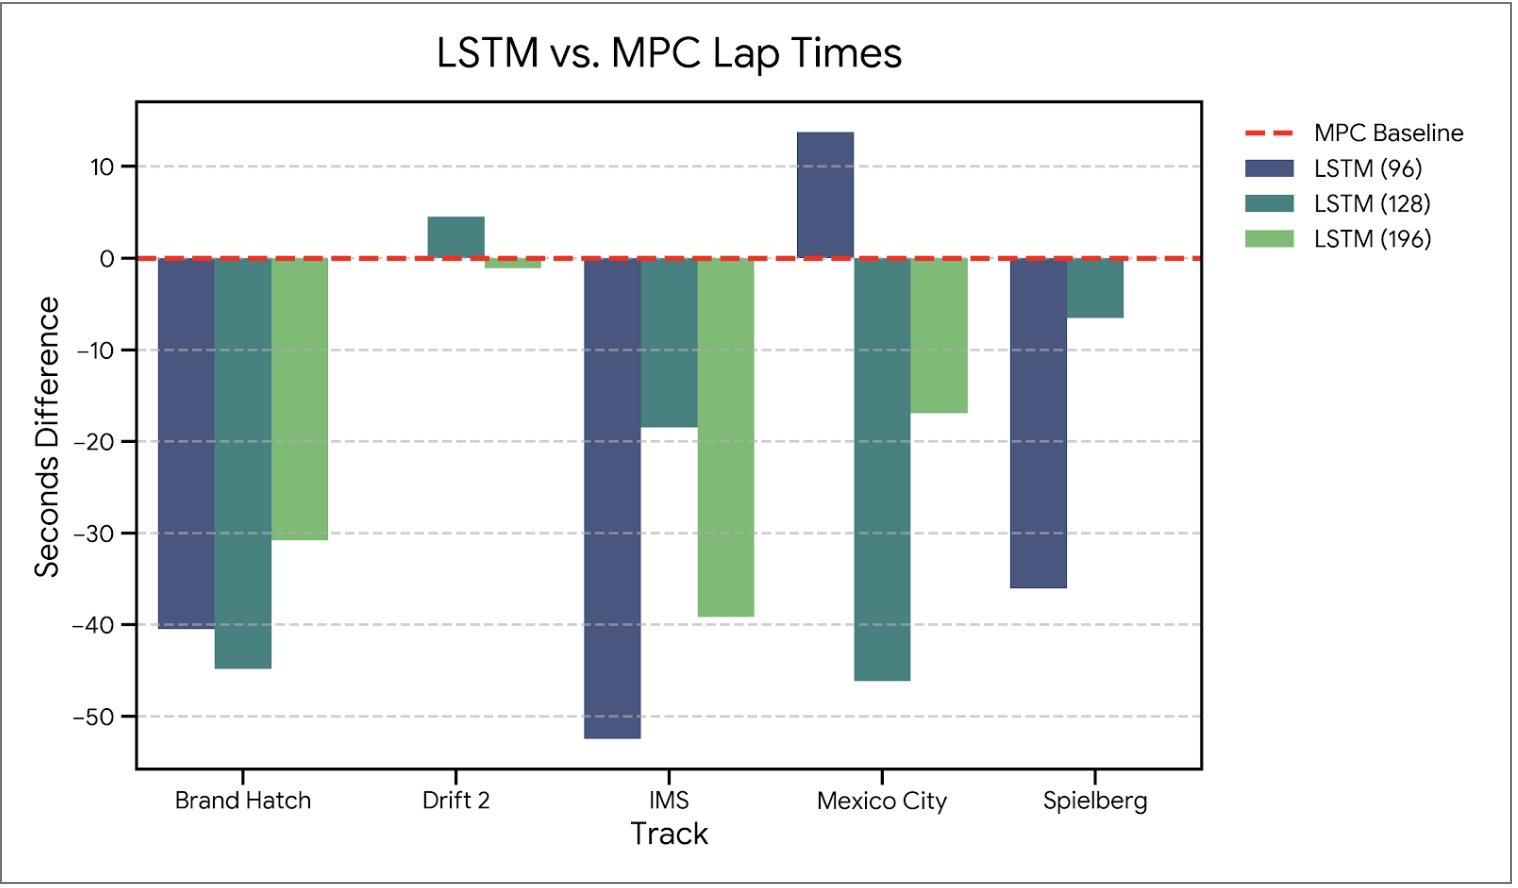
\includegraphics[width=\linewidth]{assets/lap_time_chart.png}
    \caption{Comparison of lap times across validation maps. Note the variation caused by logger discretization.}
    \label{fig:lap_times}
\end{figure}

\begin{figure}[htbp]
    \centering
    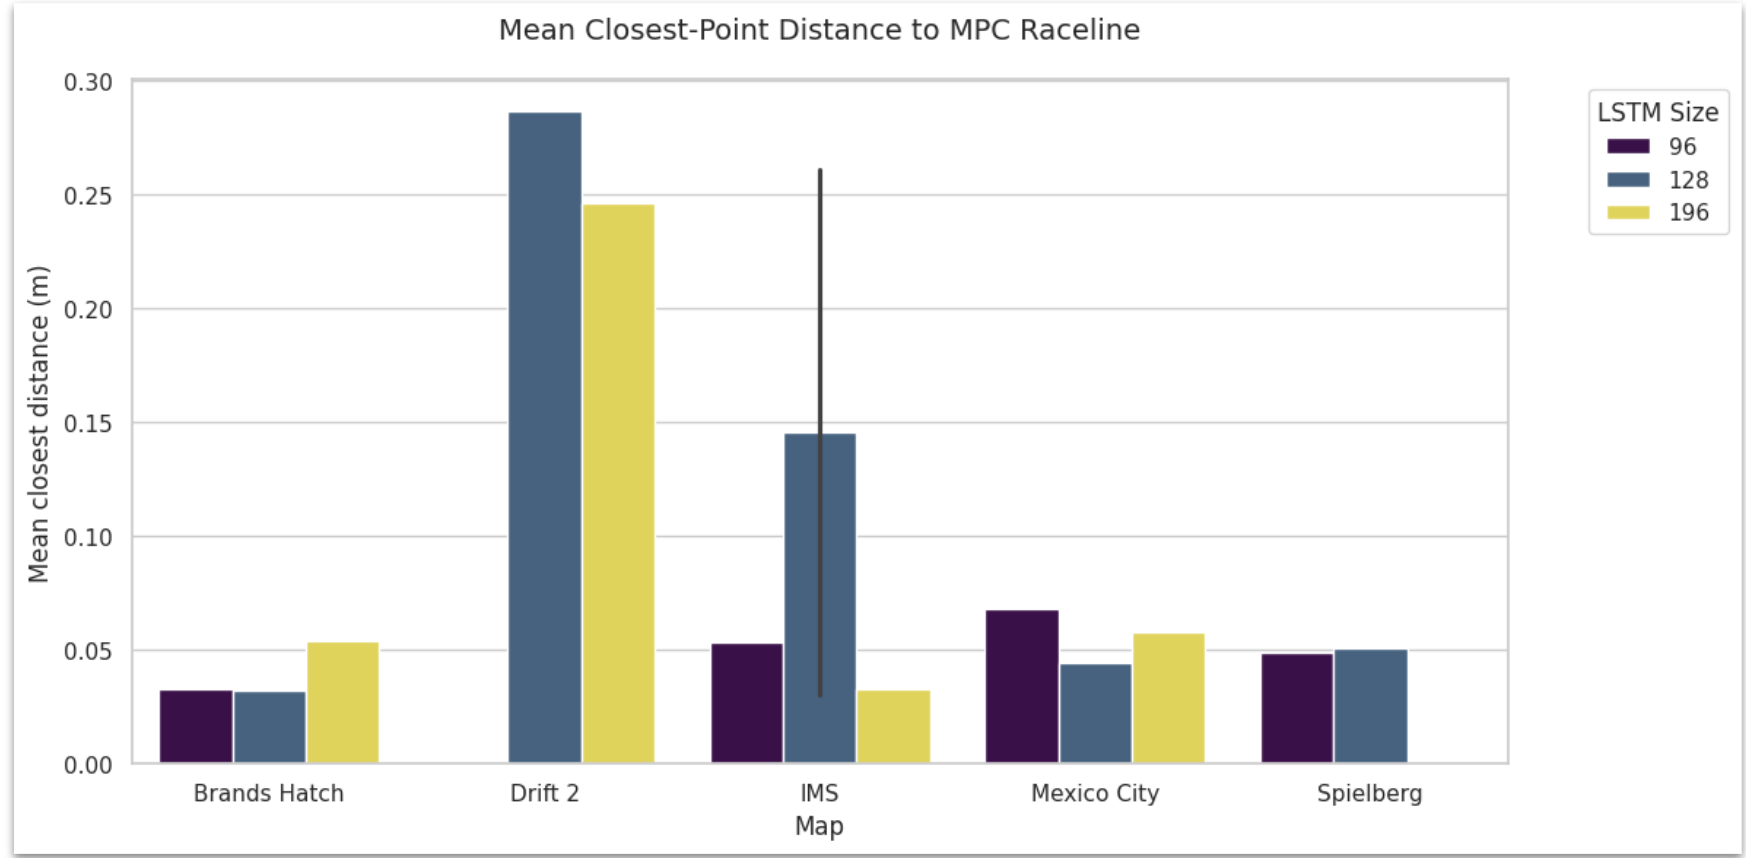
\includegraphics[width=\linewidth]{assets/raceline_optimization_chart.png}
    \caption{Mean spatial deviation (in meters) between the LSTM and MPC racelines.}
    \label{fig:raceline_optimization}
\end{figure}

\subsubsection{Computational Validation}
%Write after initial outline of validation is discussed.
%Mention how test was setup if needed

%- Charts for types of latency 

%Discuss latency

%- memory chart 

%Discuss Memory 

%Mention the preliminary nature of these results.
%Mention how some could be improved with TensorRT deployment on device. 
The primary motivation for distilling an MPC into a neural network is the drastic reduction of computational latency at runtime. To validate this, we isolated the computational overhead by running a ROS-based testing environment and extracting detailed performance profiles for both the ROS-based MPC and the ROS LSTM.

As shown in Fig. \ref{fig:latency}, the LSTM policy demonstrated significantly lower latency compared to the traditional MPC. During our trials on the IMS and Spielberg maps, the LSTM model achieved a mean end-to-end callback latency of approximately 0.74 ms per control step, compared to the MPC's 1.38 ms. More impressively, the core compute time, isolating the ONNX inference against the MPC solver, showed that the LSTM is nearly 10x faster (see Fig. \ref{fig:compute_time}). The ONNX inference averaged just 0.115 ms, while the MPC solver required 1.215 ms per step. The P95 latency for the LSTM was measured at 1.06 ms, which remains well within the strict bounds required for safe, real-time autonomous racing at 100 Hz.

\begin{figure}[htbp]
    \centering
    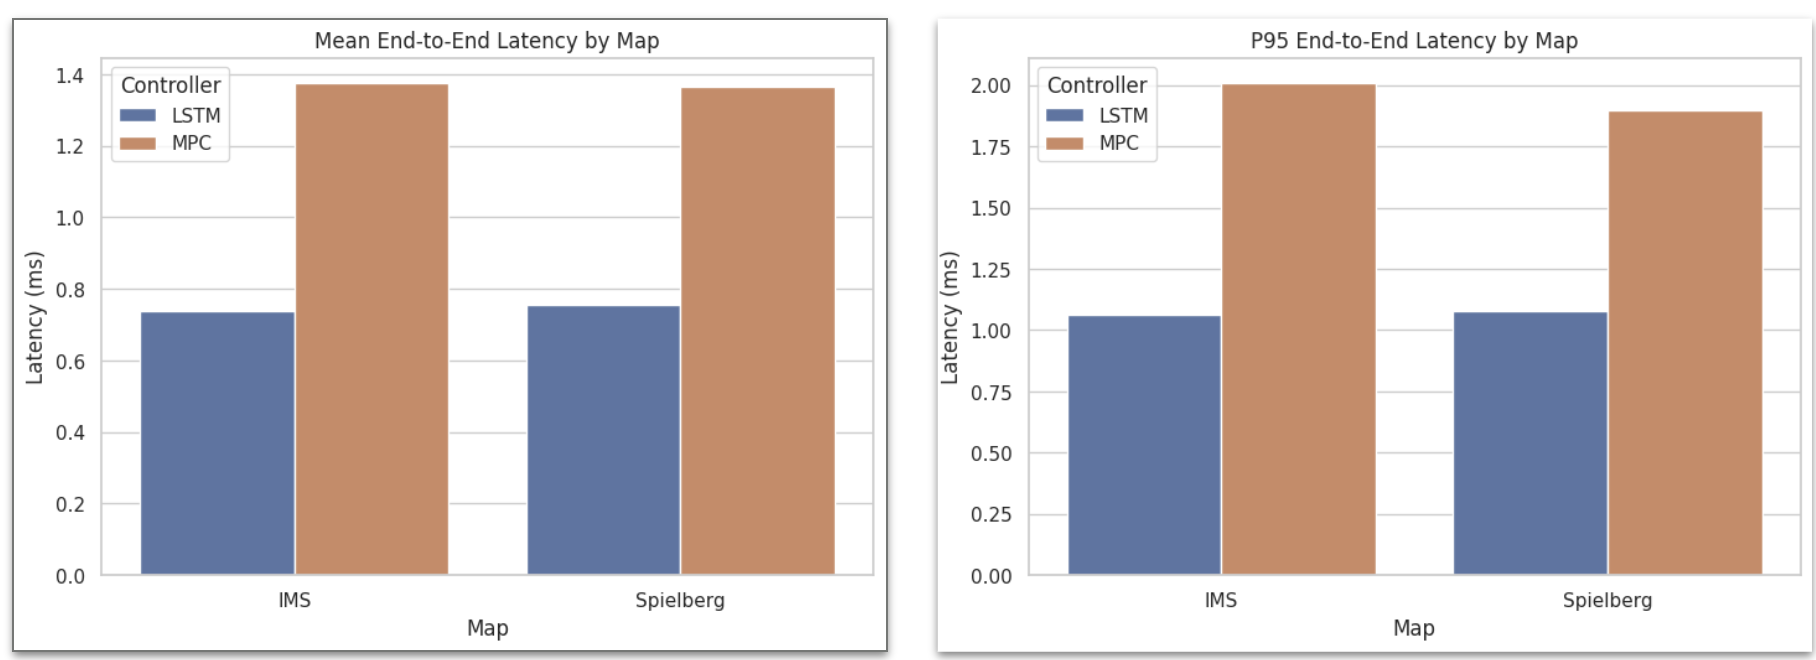
\includegraphics[width=\linewidth]{assets/latency_chart.png}
    \caption{Mean end-to-end and P95 callback latency by map.}
    \label{fig:latency}
\end{figure}

\begin{figure}[htbp]
    \centering
    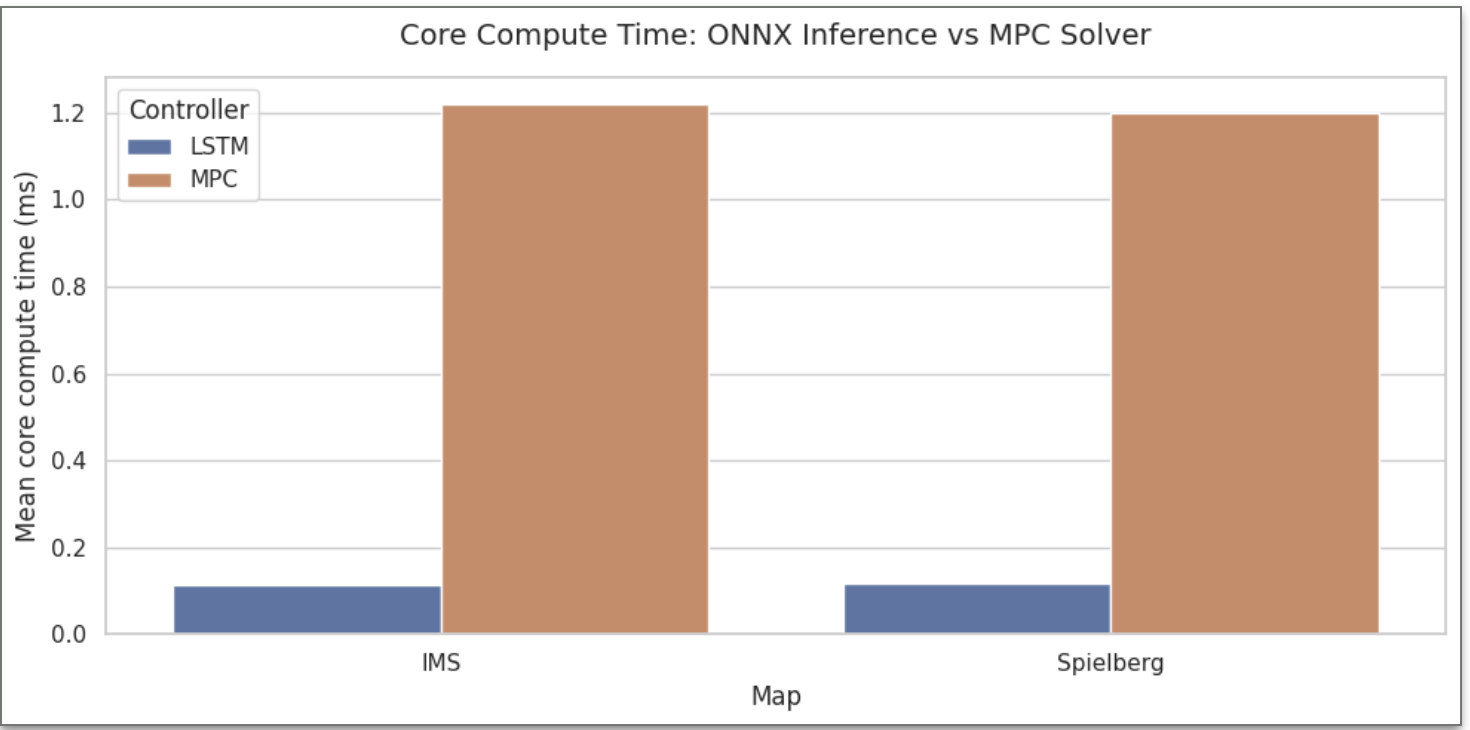
\includegraphics[width=\linewidth]{assets/compute_time_chart.png}
    \caption{Core compute time comparison: ONNX inference vs. MPC solver.}
    \label{fig:compute_time}
\end{figure}

Beyond pure speed, we evaluated the memory requirements of the sequence model, as illustrated in Fig. \ref{fig:memory}. The peak memory footprint (RSS) for the LSTM node was measured at 134.71 MB. Althou gh this is higher than MPC 85.34 MB, it remains well within the resource constraints of embedded edge hardware such as the Jetson. These results represent a baseline execution using standard ONNX; we anticipate even further reductions in latency once the model is natively compiled and deployed via TensorRT on the physical vehicle hardware.

\begin{figure}[htbp]
    \centering
    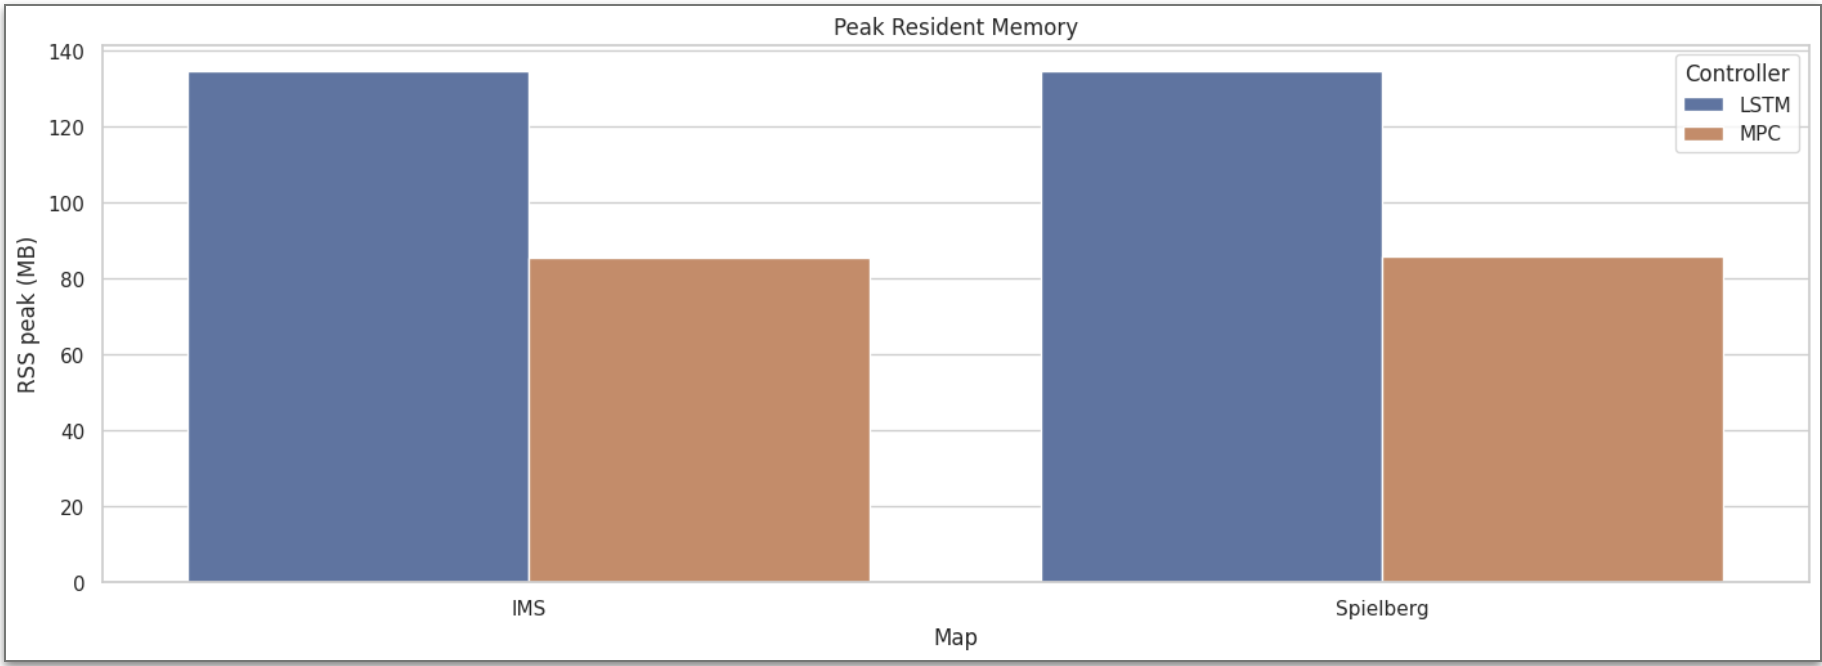
\includegraphics[width=\linewidth]{assets/memory_chart.png}
    \caption{Peak resident memory footprint (RSS) during continuous evaluation.}
    \label{fig:memory}
\end{figure}


\section{Conclusion}
%??? Was there supposed to be something here?

\section{Discussion}

Although the results demonstrate the viability of distilling MPC into a lightweight sequence model, several limitations impacted the evaluation of this approach. A primary limitation comes from our dependence on Gym-Khana for data generation. Gym-Khana proved to be highly advantageous for its rapid iteration speeds and highly configurable map sweeps.However, Gym-Khana relies on a mathematical solver (\textit{acados}) that does not easily integrate with ROS. Furthermore, the specific 'teacher' algorithm used to generate our dataset was a Spatial-Temporal MPC (STMPC), which differs slightly from the standard ROS MPC we used later for our latency baseline.

Due to this environment gap, the race performance comparison is not a perfectly direct 1:1 evaluation. We were forced to use two distinct MPC models in all our testing: the Gym-Khana STMPC was used to evaluate raceline trajectories and lap times, while a separate ROS-based MPC was used to evaluate computational latency. Consequently, performance metrics and computation metrics exist in slightly different simulation contexts.

Furthermore, this study was entirely limited to software simulation. Lacking physical hardware validation on the actual F1Tenth vehicle, we had to rely heavily on our simulated latency and memory metrics. Although these metrics attempt to compensate by approximating how the model will perform on edge hardware, they cannot fully replace physical testing constraints.

\section{Future Work}

Moving forward, future work should focus on bridging environmental gaps and expanding the tested model architectures. 

In unifiying the baseline controller, the data generation pipeline should utilize a Kinematic MPC (KMPC) bicycle model from the very beginning. Although Gym-Khana should absolutely be retained for its excellent data generation capabilities, future iterations must add support for a Gym-ROS bridge to ensure seamless transitions between data collection and validation. On the data side, the data set can be further enriched by incorporating explicit speed control directly into the raw data logs.

Architecturally, the model search space must be expanded to properly benchmark performance. Although this study focused on LSTMs, future research should implement and evaluate other sequence models,specifically Gated Recurrent Units (GRUs) and vanilla Recurrent Neural Networks (RNNs). Comparing these architectures directly with the LSTM baseline will help determine the optimal trade-off between parameter size, memory retention, and inference speed.

Most importantly, the ultimate next step is hardware deployment. Running the networks on the physical F1Tenth vehicle will provide the definitive, real-world latency and computational metrics required to fully validate the ApproxiMPC architecture.

\bibliographystyle{ieeetr}
\bibliography{references}

\appendix

Github Repo: \url{https://github.com/henry-feldhaus/F1Tenth_ApproxiMPC} 
\end{document}
